\documentclass[thesis.tex]{subfiles}
\begin{document}
\chapter{Introduction}

%\todo{%
%  This chapter should introduce:
%  \begin{itemize}
%  \item Introduce the thesis.
%  \item State the main contributions.
%  \end{itemize}
%
%  We should also ask \emph{what is the thesis of the thesis} which is a fiddly
%  way of asking what are we trying to prove with this document?
%}

\begin{figure}
  \centering
  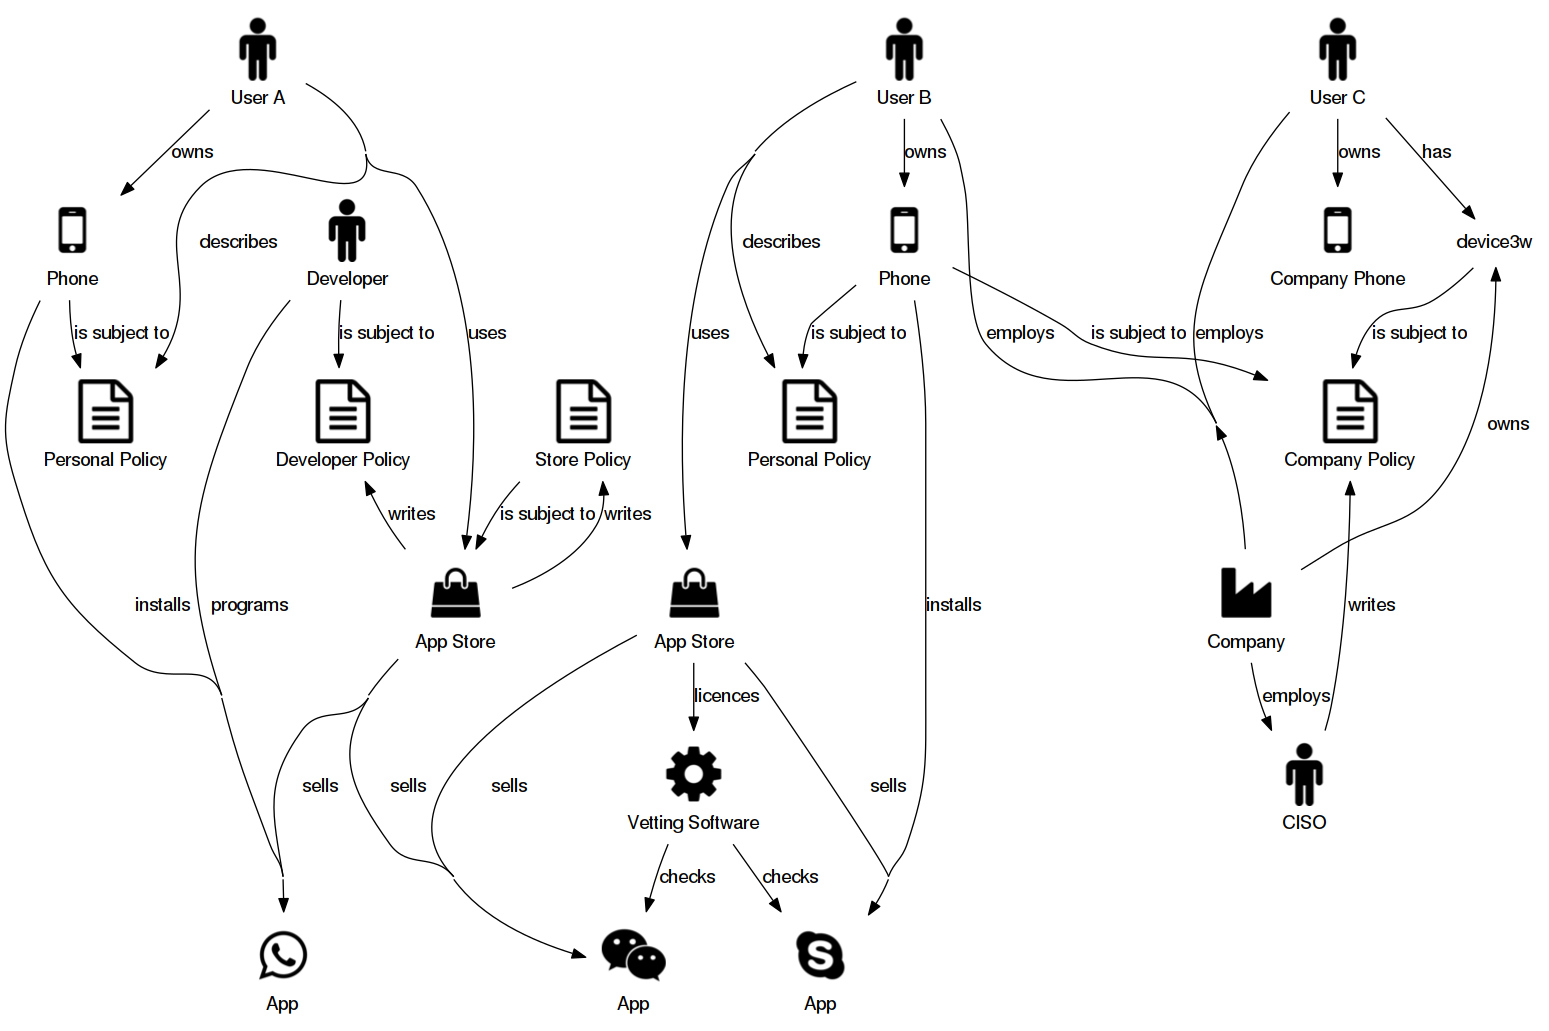
\includegraphics[width=\linewidth]{figures/mobile-ecosystem.png}
  \caption{Interactions surrounding the use of mobile devices.}
  \label{fig:mobile-ecosystem}
\end{figure}

Mobile devices are ubiquitous, yet the relationships between their users, and
the environment they run in is often vague. Users have preferences for the apps
they use. Stores have terms for the apps they sell, and for the users who buy
them. Companies have policies as to what apps and devices employees can use in
the office. The precise trust relationships, however, are often hidden in
informal, or natural language, descriptions of the policies.

As the devices have become more powerful, there has been an increasing wish to
control the devices. Companies expect devices to follow their corporate policies
within their networks and trust users to abide by their policies as well as use
tools to enforce some aspects of them. Some users may have reservations about
what data an app can get access to and may wish to restrict the app's access.
Users may rely on stores to vet the apps they sell, but will likely not know (or
necessarily care) precisely how the store checked the app.

These devices exist within the \emph{mobile ecosystem}: which we define as
\textbf{the interactions surrounding the use of smart phones and tablet
computers in a given setting}. Figure~\ref{fig:mobile-ecosystem} shows some relationships
between devices, their users and their preferences, the stores, companies and
all these principal's policies. Users have phones or other mobile devices. The users
may own personal or have company provided devices. They may have their own
preferred ways of using the device, or they have to follow policies written
by their employer. Users download apps, written by developers from app stores,
all with their own policies and some stores may delegate some aspects of
their quality control to external vetting software.

Prior work focused on how systems and tools can check and enforce more
sophisticated policies and ever finer controls. This thesis asks a different
question: \textbf{how can we capture the informal policies and trust
relationships surrounding the mobile ecosystem and use formal languages to model
and examine them?} We ask how can we tie the top-level goals in the natural
language policies and preferences to the tools used to implement them? How can
we compare different policies and highlight similarities and differences between
them precisely?

\section{The Policies of the Mobile Ecosystem}

As mobile devices are increasingly capable and hold ever-increasing amounts of
information, users and businesses need to manage how the devices behave.
Employees now bring their mobile devices to work and use them to access company
email and documents. In response to this companies might \emph{mandate} that
employees follow mobile device policies that describe how the employees should
use their devices within the company. These policies vary in terms of formality
inside and outside of a company. 
They may also use \ac{MDM} software, tools which allow companies to configure
mobile devices remotely, to enforce the policies. Regulation, such as
\ac{HIPAA}, may also affect some companies.

A user may never write their personal privacy preferences in a formal language
but they may make decisions guided by them. An example might be a user choosing
which apps to install and which to avoid, based on their own \emph{discretion}.
They may make decisions based on what their friends have told them, or what a
review said about the app.

In this section we will start to introduce by example AppPAL: an authorization
language for the policies of the mobile ecosystem, based on
SecPAL~\cite{becker_secpal:_2006}. We will describe AppPAL in greater detail in
\autoref{chap:apppal} and throughout the thesis. We have implemented SecPAL to
explore its use and build our own policy language called AppPAL to capture the
policies of the mobile ecosystem. Moreover, when we show an AppPAL snippet in
\framebox{\texttt{teletype font}} it can be parsed and used as part of a
policy\footnote{Sometimes with minimal edits as some constraints used are not
implemented.} with our \emph{AppPAL} interpreter (described in
\autoref{chap:apppal}).

A key aspect of the mobile ecosystem is \emph{delegation}. The user of a mobile
device (typically) first logs on to a Google or Apple account before using the
device, which fetches all their data from wherever server stores it. Rather than
keep account information locally an app may prompt the user to log in,
delegating to a third-party (such as Google or Facebook) to manage the account
ID. Capturing these trust relationships as policies can help clarify the precise
terms for authentication and who each principal trusts to make what decisions.
For example, an app might trust Google to manage accounts. Google will only
authorize a user if the user has authorized the app, and will only allow the app
access to the data the user has explicitly authorized:

%\noindent\begin{minipage}{\linewidth}%\vspace{\baselineskip}
\begin{lstlisting}
'app' says 'google' can-say 
  'app' canLink(User:U, Account:A).

'google' says App:A canLink(User:U, Account:Acc)
  if U hasAuthorized(A), U hasAccount(Acc).

'google' says User:U can-say U hasAuthorized(App:A)
  if U isAuthenticatedWith(Token), Token isValid.

'google' says User:U can-say App:A canAccess(Data:D)
  if D isOwnedBy(U).
\end{lstlisting}
%\end{minipage}

Users may install apps manually themselves, but they might also buy and download
apps from one or more app stores. They trust these app stores to sell them
\emph{good and safe} apps, and delegate the checking of them to the store.
Whereas, in the earlier days of PCs, a user might once have done the check
themselves (or at least delegated to an \ac{AV} package on their computer) now
the responsibility is with the stores. Now most apps come signed either by the
developer who created it (in the case of Google's Play Store), the store that
sold it (in the case of Amazon's app store) or both (Apple's App Store). These
signatures ensure integrity and some measure of authenticity, standing for an
assertion that the signer makes that the app is safe to run. For example we may
take Apple's signature as an assertion that Apple's vetting process has approved
the app is safe to use by its customers. A store may delegate to a third-party
app vetting service to assess what apps are safe (Yandex and Aptoide stores), or
use their own in-house teams.

Users sometimes recommend apps to each other. We can capture, for example, that
Alice may trust Bob to tell her which apps are good.
%
\begin{lstlisting}
'alice' says 'bob' can-say App:A isGood.
\end{lstlisting}
%
Some may consider what apps they want to use on their phone and come up with
informally applied personal policies that describe how they want to use them.
They may never write these policies down, but they might take the form of
preferences that influence the apps they choose, by capturing these we can start
to examine and compare policies as well as potentially enforcing them. Bob might recommend any app by Nintendo:
%
\begin{lstlisting}
'bob' says App:A isGood
  if A isGame,
     A hasDeveloper('nintendo').
\end{lstlisting}
%
Bob might trust reviews and review sites to give him an idea of an app's quality. 
%
\begin{lstlisting}
'bob' says App:A isGood
  if A hasReviewScore(N)
  where N > 60.
 
'bob' says 'metacritic' can-say
  App:A hasReviewScore(Percent:N).
\end{lstlisting}
%
Bob might also recommend an app based on its app store categorization and its permissions.
%
\begin{lstlisting}
'bob' says App:A isGood
  if A hasCategory('flashlight'),
     A hasPermissions(P)
  where ! contains(P, 'INTERNET').
\end{lstlisting}

They allow their employers to say how they should their devices, who
may in turn delegate to IT departments, to write rules, which may
delegate back to the users to state what rules they're willing to
follow.

A company looking to control their employee's mobile devices at work
might write a \ac{BYOD} policy that their employees agree to
follow. They might also use \ac{MDM} software to control some aspects
of their devices. The company might write these with varying degrees
of formality but often they use natural language. This adds vagueness
and can lead to confusion about how the company upholds the policy. By
describing the policy in a formal language we can express the policy
rigorously. We can start to make comparisons between users, and with
rules for checking the policy start to help the user to make decisions
more accurately, or measure the extent a user follows their stated
policy. Using formal languages we can model the policies precisely,
helping clarify their meanings and make precise comparisons between
different policies. We could tie the rules in the \ac{BYOD} policies
to the \ac{MDM} tools used to check them.

If a company needs to use apps which conform with a policy such as
\ac{HIPAA} they could use static analysis tools to check for some
aspects of the policy.  A company might use
Mallodroid~\cite{fahl_why_2012} to detect when apps send data unencrypted.  
%
\begin{lstlisting}
'company' says Employee:E canUse(App:A)
  if A isHIPAAConformant
  where
    mallodroidCheckSafe(A) = True;
\end{lstlisting}
%
It is important not to confuse the tools and
techniques we might use to uphold parts of a policy with the end
goal of ensuring compliance.  A formal language that
lets us sever the policy from its implementation can help us
understand the policy precisely, and then show precisely how we check the
policy.  It lets us see which tools are checking what rules, and identify gaps where the policy is not
being checked sufficiently.

These trust relationships and delegations permeate the entire mobile
ecosystem.  They represent an important aspect of the ecosystem that a
policy language should catch to describe the
relationships and policies within it.


In this thesis we will come back to these ideas of user's personal
privacy policies and BYOD policies as they show two different aspects
of how policies are used within the mobile ecosystem.
%
User's privacy preferences are very informal and may not be something
a user would ever consider writing down.  Rather, a user's privacy
preferences guide which apps they might use. A user might even be
willing to use an app that does not match their preferences in some
cases, such as using the Facebook app (which can access lots of data
on a user's device) whilst being generally unhappy sharing their data
with their software.
%
In contrast a BYOD policy can exist as a formal agreement (though
often \emph{informally} specified) between the company and its
employees.  An employee might reasonably expect to face consequences
if their employer discovers they broke the BYOD rules.

Superficially these policies also resemble classic DAC and MAC
policies: the company \emph{mandates} the BYOD policy, the user uses
their \emph{discretion} when picking the apps they use on their phone.
An interesting aspect of the mobile ecosystem is that the policies are
more complicated than simple MAC and DAC distinctions and use aspects
of both.  In \autoref{chap:byod} we will look at how companies use
employee's discretion to judge if aspects of the company's BYOD
agreements (such as ethical policies) have been followed.  A user who
uses a tool, such as a \emph{fine grained permissions system} (such as
one described in \autoref{sec:fine-grained-permissions}) or create a
curated app store (we give a method to do so using a policy in
\autoref{sec:an-apppal-enhanced-store}), will end up writing a
MAC-style policy describing how their phone should behave or what apps
the store should sell.

BYOD policies and privacy preferences are only of a subset of the
policies we might see in the mobile ecosystem.  We will survey some
other policies in the course of the thesis including app store terms
and conditions, and the app signing models built into the mobile OSs,
but we chose to focus on BYOD and privacy preferences as they covered
a range of policy styles, high and low-level policy topics and could
showcase some of what makes the mobile ecosystem fascinating.

\section{Thesis Outline and Publications}

The rest of this thesis is organised into the following chapters.
Some work described has been presented at various conferences, workshops and PhD symposiums through the course of the PhD.
We describe the publications, and show where they fit into the various chapters.

\begin{itemize}
\item \textbf{Chapter 2: Background.} 
  Describes Becker~\etal's work on SecPAL, and gives an overview of work developing policy languages.

\item \textbf{Chapter 3: Instantiating and Evaluating SecPAL.} 
  Introduces AppPAL as a language instantiating SecPAL to describe the policies
  of the mobile ecosystem. We introduce the language through examples before
  showing how we implemented it. We also describe some modifications to the
  language from SecPAL to make writing policies easier. We conclude by describing
  our tools for analyzing AppPAL policies for satisfiability and redundancy
  errors.
  
  Some early examples were taken from our paper:
  \begin{itemize}
  \item\emph{Towards an authorization framework for app security
      checking~\cite{hallett_towards_2014}.} A PhD symposium paper describing how
    we might use SecPAL to model policies in the mobile ecosystem.
  \end{itemize}

\item \textbf{Chapter 4: App Stores and App Preferences.} 
  Having described AppPAL, start to describe the differences betweeen different
  app stores and survey their different terms and conditions. We use AppPAL to
  capture descriptions of user's app privacy preferences; and measure the extent
  users follow these preferences when selecting apps by comparing with records of
  user's app installation history. Finally, we describe a tool for generating
  \emph{curated} app stores on the basis of a policy.
  
  The implementation described, and work on capturing user's privacy preferences is included in our papers:
  \begin{itemize}
  \item\emph{AppPAL for Android~\cite{hallett_apppal_2016}.} Describes AppPAL as an instantiation of SecPAL.  Presents evaluation algorithm.  Shows how to capture user privacy preferences as AppPAL policies and tries to find examples of users following the policies in a user app-installation dataset.
  \item\emph{Poster: Using Authorization Logic to Capture User Policies in Mobile Ecosystems~\cite{hallett_poster:_2015}.}  Presents early work measuring the extent users seem to follow an AppPAL translation of user privacy prefences.
  \end{itemize}

\item \textbf{Chapter 5: Applying AppPAL to BYOD Policies.}
  We move from describing \emph{user-centric} policies, to ones companies might
  want to enforce. We look at how we can capture BYOD policies using AppPAL by
  looking at five BYOD policies (which are given in Appendix A). In capturing the
  policies, we identify two idioms that existing MDM tooling does not capture. We
  also describe how AppPAL could be used to enforce a BYOD policy by integrating
  with existing tooling.
  
  This chapter encompasses and extends our work presented in:
  \begin{itemize}
  \item\emph{Capturing Policies for BYOD~\cite{hallett_capturing_2017}} Describes work on using AppPAL to capture the rules and trust relationships in BYOD policies.
  \item\emph{Common Concerns in BYOD Policies~\cite{hallett_common_2017}.} Describes work looking at BYOD policies to find common areas of concern.  
  \item\emph{Specifying BYOD Policies with Authorization Logic~\cite{hallett_specifying_2016}.} PhD symposium paper describing early work capturing BYOD policies with AppPAL.  Shows how we could use AppPAL to look for common problems, such as completeness.
  \end{itemize}

\item \textbf{Chapter 6: Future Work.}
  Describes possible future work, including a probabilistic variant of AppPAL.
 
\item \textbf{Chapter 7: Related Work.} 
  Describes XACML and DKAL, to related policy languages. We also give an overview
  of the various \emph{fine-grained permissions systems} for Android that can be
  used to enforce some policies.
\end{itemize}



\end{document}


%%% Local Variables:
%%% mode: latex
%%% TeX-master: "../ch1"
%%% End:
